\chapter{INTRODUCTION}
\label{sec.introduction}
Broadband Internet access for home use is rapidly evolving. The United States
alone has
more than 279 million broadband users. The number of Internet users in other regions is even more
impressive, with China counting more than 641 million.~\cite{asia}. Yet, despite its
pervasiveness, little is known about most home networks\lois{What do you need to know
that we don't know now? Is it power usage? Interaction with individual systems?
You have to be specific}. This lack of knowledge hampers progress in
a number of important research areas, from ISP performance to large-scale
topology mapping and wireless network utilization.

Researchers, policymakers and Internet Service Providers (ISPs) are also eager to
learn more about emerging technologies made possible by these networks.
"Smart homes," in which devices from thermostats to door locks can be controlled
remotely \lois{Notice what I included in this sentence. That is the type of
detail needed} are now exciting realities. In 2016, 4 billion
new objects (e.g., laptops, handhelds, interactive television, wireless
based security cameras) will become available to consumers~\cite{gartner}.

But with the benefits of these products also come concerns. For these devices to
 work, they usually need to be connected to a wireless router. If a router
 is compromised via buggy software, it is possible that hackers could unlock
 not only critical data, but also
  your front door. Therefore, as their use grows, understanding vulnerabilities in both routers and
broadband networks becomes crucial in order to prevent these types of attacks.
Due to these changes, the value of studying home networks for researchers, policy
 makers and ISPs continues to grow.

 At this point in time studying home networks on a large scale has been
  difficult because network technologies, such as network address translators (NATs),
   present only an opaque view of the home network to the global Internet. \lois{you
   need to use a better word than "opaque." I would change it, but I don't know
   what you mean by it.To better understand the behavior of networks, a
    formal study using an experimental platform
that can gather data via from homes  is needed to provide
visibility into the missing part of Internet.\lois{Think about rewording that last
part. What do you mean by "the missing part of the Internet?" What is missing from?}
Such a platform should also provide a set of programming interfaces to support
as wide an array of measurements as possible, including factors affecting broadband
 performance, or data that can increase understanding of usage and connectivity in home networks.
 Lastly, the ideal platform proposed here should ensure the privacy of the user
 and prevent abuse of his or her device or network resources.

A number of measurement and experimentation platforms have been developed to
support controlled network experimentation
and broadband characterization for home
 networks, including
BISmark~\cite{183951}, Samknows~\cite{samknows} and Dasu~\cite{
sanchez2014measurement}. \lois{maybe more information on these platforms}
However, the process of vetting BISmark
experiments is manual, which will be a limiting factor a deployment
grows. \lois{explain sentence above. Who or what is involved in vetting an
experiment?} SamKnows has deployed on thousands of home routers in the US and the UK,
but only supports limited performance measurements. Dasu is a host-based
software client, thus it is not able to run certain measurements. If the hosts are
turned off, measurements stop, it cannot run continuous measurements.

In this paper, we introduce \sysname, a distributed cloud platform that allows
researchers to run both active and passive experiments securely from a wireless router
on a home network. Through a programmable interface on the device, the platform enables researchers
to deploy a wide range of network measurements from a
vantage point between the access ISP and the home network, as shown in Figure~\ref{figure:design}.
Researchers can access and compile data on systems worldwide, while preserving
the user's privacy, and securing the device itself. The information gathered from
 such studies could assist users in evaluating the services
they are paying for, researchers in understanding the factors impacting
performance, and ISPs in finding ways to improve their service.

\sysname
implements a number of measurement primitives to enable researchers,
policy makers and Internet Service Providers (ISPs) to program network measurements.
\lois{what do you mean bY program network measurements? Is it setting limits on these measurements?
recording them?}To protect device availability and privacy, \sysname supports a very flexible
  language for experiment specification based on Repy, a lightweight,
 Python based, performance isolation and extensible programming
  language~\cite{cappos2010retaining}. Because it is designed for running
  measurement software on a home access point, a platform
  like \sysname has a number of unique strengths and challenges.
First, software must be small and easy-to-deploy because \sysname is deployed
on resource-constrained devices. Second, \sysname sits on the direct path of real
  Internet users. Any buggy or malicious experiments could be able to disrupt
  Internet connectivity. Thus it must guarantee that a poorly designed experiment
  can not negatively effect a user's Internet connection. Third, it is important
to make the system robust by providing remote maintenance and updates because
    of the unmanaged complexity of its home network environments. Finally, \sysname
must provide a rich set of APIs for a variety of network measurements.


\begin{figure}%[h]
\centering
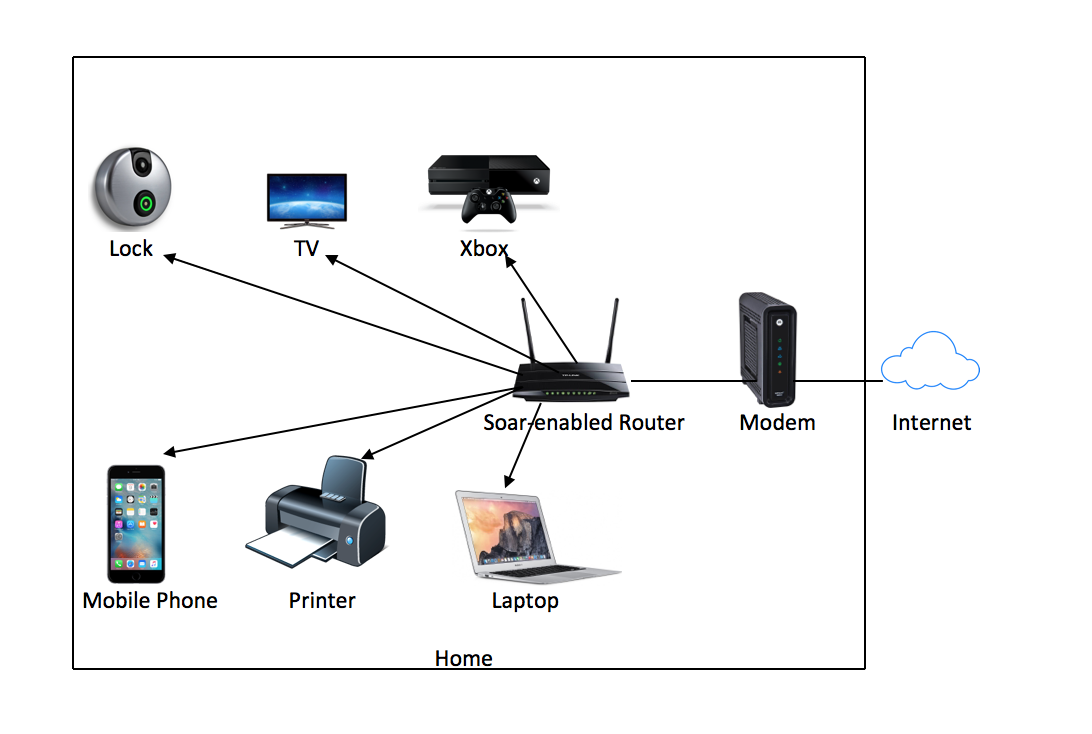
\includegraphics[width=0.8\columnwidth]{figure/home-network.png}
\caption{The SOAR-enabled router sits on the direct path of real
Internet users. It supports both active and passive network measurements.}
\label{figure:design}
\end{figure}


The primary contributions of this study are as follows:
{\raggedright
\begin{itemize}
\item\textbf{1) Home routers platform deployment:} This platform is based on
the Seattle testbed, a community-driven and open-source cloud computing
system~\cite{zhuang2013experience}~\cite{cappos2009seattle}. Compared to computer
 and mobile device environments, deployment on a home wireless router has more
 resource limitations, such as restricted computational resources. However,
 recently we have been able to port Seattle Testbed to OpenWrt, a popular Linux
 platform for home routers\cite{openwrt}. Users can build their own \sysname
 installer (IPK) via config file we provide using OpenWrt SDK and install it on the device directly.

\item\textbf{2) Extensions to Seattle Testbed:}  Our testbed implements new
research capabilities for home wireless routers by improving on the Seattle sandbox.
To handle home wireless routers, our testbed uses low-level system calls in
the OpenWrt platform with Restricted Python (Repy)\cite{cappos2010retaining},
the core sandbox of Seattle. In order to securely interact with home routers on
remote user devices, we use Fence (a non-intrusive mechanism that mediates and
 limits access to diverse resources using uniform resource control)~\cite{li2015fence}
 to allocate a fixed percentage of the device's CPU, memory disk, and other resources
  to one or more VMs. For example, we set the legal times of accessing the \emph{/proc}
  file system to prevent DoS attacks using our API calls. Our testbed adds eight functionalities
   based on Repy, including \texttt{get\_network\_bytes}, \texttt{get\_network\_packets},
    \texttt{get\_network\_interface}, \texttt{wifi\_status}, \texttt{scan},
     \texttt{get\_station}, \texttt{ping} and \texttt{traceroute}. This rich set
      of measurement primitives can help researchers implement a wide range of
      network measurements, such as mapping Internet paths (via traceroute),
      studying home network usage patterns, and understanding wireless network performance.

\item\textbf{3) Experimental characterization of home wireless networks:} By
integrating \sysname into home networks, we get the benefits of a real world
deployment while ensuring flexibility to run experiments without compromising
home networks. We demonstrate \sysname's utility by implementing hybrid measurements
 that together exercise different new API calls (e.g, \texttt{get\_network\_bytes},
  \texttt{get\_network\_interface}, \texttt{wifi\_status})

   \item\textbf{4) Characterizing home wireless performance from gateway view:}
  We monitor our lab's network traffic, which is in an office building, from the
  vantage point of the access point. We report on additional experiences gained
   using \sysname in three different use cases. We find that there are many
   factors affecting throughput on 2.4 GHz and 5 GHz band.
   We also find that most of access points select non-overlapping channels
    (e.g., channel 1, 6, 11) to avoid adjacent-channel interference.
\end{itemize}
\par}
The rest of this thesis is structured as follows. We discuss related work and
the motivation for our research in \S{\ref{sec.relatedwork_motivation}}.
In \S{\ref{sec.goals_challenges}}, we point out the goals and challenges of our work.
 \S{\ref{sec.design}} and \S{\ref{sec.implementation}} describe the design and
 implementation of \sysname and characterize our current deployment. We present
 three study cases to illustrate the benefits of an experimental platform that
 run on the home wireless router in \S{\ref{sec.evaluation}}. Finally, we discuss
 future work and conclusions in \S{\ref{sec.conclusion}}.



Currently it has been difficult to study home
  networks on a large scale because network technologies like network address translators (NATs) present only an opaque view of the home network to the global Internet. To better understand home networks, an experimental platform should be hosted in home networks, to provide visibility into the missing part of Internet.  Such a platform also should provide a set of programming interfaces that support the implementation of as wide an array of measurement as possible, such as studying factors affecting broadband performance or understanding usage and connectivity in home networks. To let participants trust us and save researchers' effort in recruiting participants, user security and privacy should be as first-order concern. Experimenters need a platform that does not compromise the privacy of the user and abuse of device or network resources.

Today's measurement and experimentation platform for home networks such as
BISmark~\cite{183951}, Samknows~\cite{samknows} and Dasu~\cite{
sanchez2014measurement} all support controlled network experimentation
and broadband characterization. However, the process of vetting BISmark
experiments is manual, which will be a limiting factor as the deployment
grows. SamKnows has deployed thousands of home routers in the US and the UK,
but only supports limited performance measurements. Dasu is a host-based
software client, thus it is not able to run certain measurements due to
application restriction and cannot run continuous measurements (i.e., since
hosts can be turned off, moved, etc.)

To address these issues, we developed \sysname, an open research testbed that implements a number of measurements primitives that enable researchers, policy makers and Internet Service Providers (ISPs) to program network measurements. \sysname is able to deploy on home wireless router so that it is capable of running both active and passive experiments from a vantage point between the access ISP and the home network, as shown in Figure~\ref{figure:design}. With this information, users could evaluate the service they are paying for, researchers could study the factors impacting performance and ISPs could improve their service. To protect device availability and privacy, \sysname supports a very flexible language for experiment specification based on Repy which is lightweight, python based, performance isolation and extensible programming language~\cite{cappos2010retaining}. It provides researchers with the ability to install sandboxed measurement applications on the home wireless router.

\begin{figure}%[h]
\centering
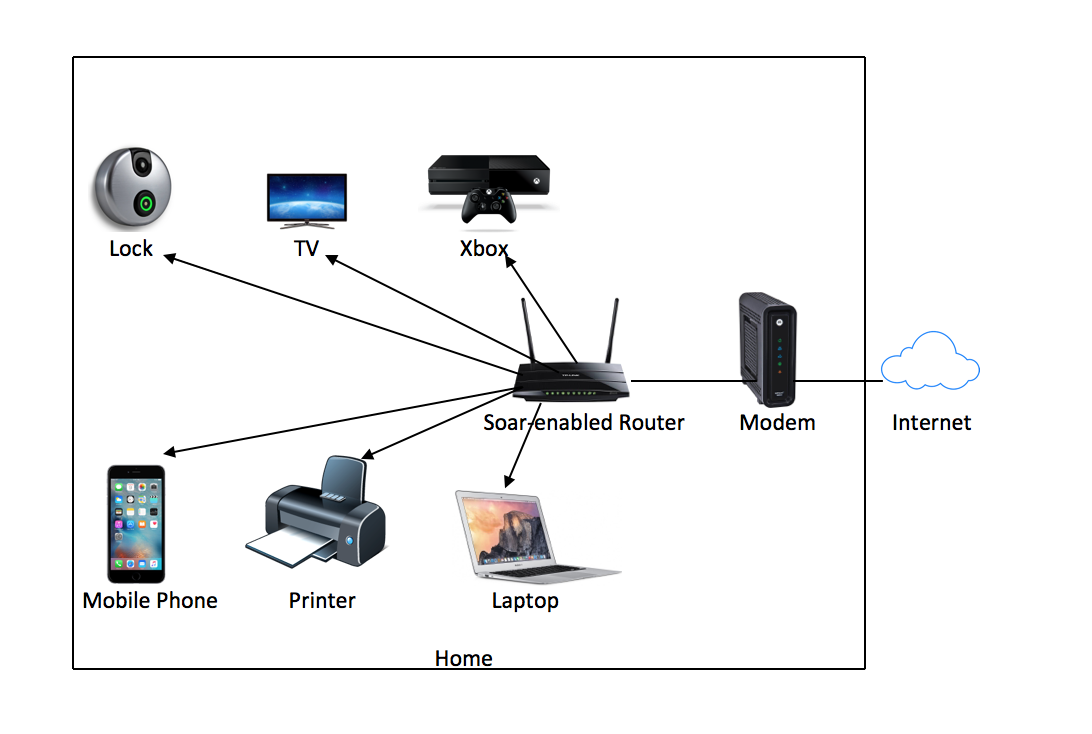
\includegraphics[width=0.8\columnwidth]{figure/home-network.png}
\caption{The SOAR-enabled router sits on the direct path of real
Internet users. It supports both active and passive network measurements.}
\label{figure:design}
\end{figure}

Both strengths and challenges of a platform like \sysname stem from
its inclusion of measurement softwares on the home gateway. First, each softwares must be small and easy-to-deploy because \sysname is deployed on resource-constrained devices. Second, \sysname sits on the direct path of real Internet users. Any buggy or malicious experiments could be able to disrupt Internet connectivity. Thus it must guarantee that a poorly designed experiment cannot bring negative effect on user's Internet connection. Third, it is important to make system robustness, remote maintenance and update because of the unmanaged complexity of its home network environments. Finally, \sysname must provide a rich set of APIs for a variety of network measurements.

In this paper, we introduce \sysname, a distributed cloud platform that allows researchers to run their project on system worldwide. This platform provides secure data access while preserving user's privacy. Due to those privacy and security mechanisms, it could be able to save researchers' effort in recruiting volunteers. Through a programmable interface on device, the platform enables researchers to deploy a wide range of network measurements including active and passive measurements. We also discuss the constraints we faced in the design, implementation and deployment of \sysname.

We make the following contributions in this work:
{\raggedright
\begin{itemize}
\item\textbf{1) Home routers platform deployment:} This platform is based on Seattle testbed, a community-driven and open-source cloud computing system~\cite{zhuang2013experience}~\cite{cappos2009seattle}. Compared to computer and mobile device environments, deployment on home wireless router has more resource limitation such as restricted computational resources. However, recently we are able to port Seattle Testbed to OpenWrt, a popular Linux platform for home routers\cite{openwrt}. Users can build their own \sysname installer (IPK) via config file we provide using OpenWrt SDK and install it on the device directly.

\item\textbf{2) Extensions to Seattle Testbed:}  Our testbed implements new research capabilities for home wireless router by improving on the Seattle sandbox. To handle home wireless routers, our testbed uses low-level system calls in the OpenWrt platform with the Restriction Python (Repy)\cite{cappos2010retaining}, the core sandbox of Seattle. In order to securely interact with home routers on remote user devices, we use Fence (a non-intrusive mechanism that mediates and limits access to diverse resources using uniform resource control)~\cite{li2015fence} to allocate a fixed percentage of the device's CPU, memory disk, and other resources to one or more VMs. For example, we set the legal times of accessing \emph{/proc} file system to prevent DoS attack using our API calls. Our testbed adds eight functionalities based on Repy, include \texttt{get\_network\_bytes}, \texttt{get\_network\_packets}, \texttt{get\_network\_interface}, \texttt{wifi\_status}, \texttt{scan}, \texttt{get\_station}, \texttt{ping} and \texttt{traceroute}. These rich set of measurement primitives help researchers to implement a wide range of network measurements, such as mapping Internet paths (via traceroute), studying home network usage pattern and understanding wireless network performance.

\item\textbf{3) Experimental characterization of home wireless networks:} By integrating \sysname into the home networks, we get the benefits of a real world deployment while ensuring flexibility to run experiments without compromising home network. We demonstrate \sysname's utility by implementing hybrid measurements that together exercise different new API calls (e.g, \texttt{get\_network\_bytes}, \texttt{get\_network\_interface}, \texttt{wifi\_status}): Characterizing home wireless performance from gateway view. We monitor our lab's network traffic which in an office building from the vantage point of the gateway. We report on additional experiences gained using \sysname in three different use cases. We find that there are many factors affecting throughput on 2.4 GHz and 5 GHz band. We also find that most of access points select non-overlapping channels (e.g., channel 1, 6, 11) to avoid adjacent-channel interference.
\end{itemize}
\par}
The rest of thesis is structured as follows: We provide related works and motivation in \S{\ref{sec.relatedwork_motivation}}. In \S{\ref{sec.goals_challenges}}, we point out the goals and challenges of our work. \S{\ref{sec.design}} and \S{\ref{sec.implementation}} describes the design and implementation of \sysname and characterize our current deployment. Then we present three study cases to illustrate the benefits of an experimental platform that runs on the home wireless router in \S{\ref{sec.evaluation}}. Finally, we discuss future work and conclusion in \S{\ref{sec.conclusion}}.
